\documentclass[addpoints]{exam}
\usepackage{url}
\usepackage{times}
\usepackage{epsfig}
\usepackage{listings}
\usepackage{mathtools}
\lstset{
basicstyle=\small\ttfamily,
columns=flexible,
breaklines=true,
escapeinside={||},
mathescape=true
}

\lhead{\ifcontinuation{Question \ContinuedQuestion\ continues\ldots}{}}
\chead{ECE 422 / CS 461, Final Exam}
\rhead{Friday, December 11th, 2015}
\lfoot{Points: \makebox[.5in]{\hrulefill} / \pointsonpage{\thepage}}
\cfoot{\thepage\ of \numpages}
\rfoot{NetID:\enspace\makebox[1.5in]{\hrulefill}}
%\rfoot{\netid}

\qformat{\thequestiontitle\dotfill \emph{\totalpoints\ points}}

\begin{document}

\begin{titlepage}
  \vspace*{\fill}
  \begin{center}
    \Large\textbf{ECE 422 / CS 461, Final Exam}\\
    \large\textit{Friday, December 11th, 2015}\\
  \end{center}
  \vspace{.5in}
  \par\large{Name:}\hrulefill\\
  \par\large{NetID:}\hrulefill\\
  \vspace{.5in}
  \begin{itemize}
  \item Be sure that your exam booklet has \numpages\ pages.
  \item Absolutely no interaction between students is allowed.
  \item Show all of your work.
  \item Write all answers in the space provided.
  \item Closed book, closed notes.
  \item No electronic devices allowed.
  \item You have \textbf{THREE HOURS} to complete this exam.
  \end{itemize}
  \vspace*{\fill}
\end{titlepage}
\newpage 

\begin{center}
  \vspace*{\stretch{1}}
  \gradetable[v][pages]
  \vspace*{\stretch{1}}
\end{center}
\newpage

\begin{questions}

\titledquestion{Question \thequestion: Multiple Choice}

\textbf{For each question, circle all that apply.}

\begin{parts}
	
\part[1]

Data on Dynamic RAM is instantaneously lost when power is cut: %-Dhruv V

\begin{choices}
	\choice True
	\correctchoice False
\end{choices}

\part[1]

Which of the following is an example of multi-factor authentication: %-Dhruv V

\begin{choices}
	\choice Being forced to have a password that is longer than 8 characters and includes a number.
	\correctchoice Withdrawing money from an ATM using a credit card and PIN.
	\choice Having to change your password every 6 months.
	\choice Having one key with access to multiple facilities.
	
\end{choices}

\part[1]

Consider the following C function signature: %-chingyang
\begin{lstlisting}
void foo(int var1, int var2, int var3)
\end{lstlisting}
In the 32-bit C calling convention learned in class, which of the following correctly describes how parameters are passed to the function?

\begin{choices}
	\choice Pushed onto the stack in this order: var1, var2, var3
	\correctchoice Pushed onto the stack in this order: var3, var2, var1
	\choice Placed in registers: var1 in EAX, var2 in EBX, var3 in ECX
	\choice Placed in registers: var3 in EAX, var2 in EBX, var1 in ECX
\end{choices}

\part[1]

In MP4, you used a buffer overflow attack to result in transferring control to your shellcode.
What did you overwrite that would result in the program transferring control to your shellcode?
\begin{choices}
	\choice Local variables
	\choice Saved base pointer
	\correctchoice Return Address
	\choice Function arguments
\end{choices}

\part[1]

If a file should have permissions read/write for owner, read for group, and write for others, what should the permission bits look like?   %- Siddharth

\begin{choices}
	\choice -rwxr---w-
	\correctchoice -rw-r---w-
	\choice -rw--w-r--
	\choice --w-rw-r--
\end{choices}

\part[1]

Malware that propogates itself without any human interaction is called: %- Siddharth

\begin{choices}
	\choice Trojan Horse
	\choice Rootkit
	\correctchoice Worm
	\choice Virus
\end{choices}

\part[1]

An attacker places the address of a series of gadgets on the stack. What is she doing? %- Siddharth

\begin{choices}
	\correctchoice Return oriented programming
	\choice Smashing the stack
	\choice Formatted string attack
	\choice Dictionary attack
\end{choices}

 \part[1] %shivam t/f

When considering onion routing, there are no side-channel attacks.

\begin{choices}
\choice True
\correctchoice False
\end{choices}

\part[1] %simon's t/f #1

\pagebreak

Confidentiality ensures anonymity.

\begin{choices}
\choice True
\correctchoice False
\end{choices}

\part[1] %simon's mc #1

Off-the-Record (OTR) messaging ensures:

\begin{choices}
\choice Anonymity
\choice Authenticity
\choice Confidentiality
\choice Deniability
\choice Forward secrecy
\correctchoice All of the above.
\end{choices}

\part[1] %simon's mc #2

Which of the followings are true about Tor?
\begin{choices}
\choice Tor works at the application layer, specifically for HTTP/HTTPS traffics.
\correctchoice The source is left anonymous because each Tor relay decrypts a layer of encryption to reveal only the next relay, the final decryption revealing the original content and the destination.
\choice One of the differences between VPN (e.g. hidemyass.com) and Tor is that Tor prevents eavesdropping at the exit node by using end-to-end encryption such as SSL or TLS.
\choice Tor provides better anonymity, privacy, and security than VPN, but it is much slower.
\choice All of the above.
\end{choices}
\end{parts}
\pagebreak

\titledquestion{Question \thequestion: Short Answer}
\begin{parts}
\part[2]

Describe the dormant phase and action phase of a computer virus. %-Dhruv V

\begin{solutionorbox}[1in]   
	\begin{lstlisting}
	Dormant - The virus is laying low and avoiding detection
	Action - The virus performs the malicious action that it was designed to perform.
	\end{lstlisting}
\end{solutionorbox}

% shivam
\part[2]

Identify an issue with onion routing and a defense for it.

\begin{solutionorbox}[1in]   
	\begin{lstlisting}
	+1 point: (attack) rubber-hose cryptanalysis of mix operators
	+1 point: (defense) use mix servers that are located in different countries

	OR 

	+1 point: (attack) the attacker/adversary operates the mixers
	+1 point: (defense) have a lot of mix servers

	\end{lstlisting}
\end{solutionorbox}

% shivam
\part[3]

Identify three access control designs.

\begin{solutionorbox}[2in]   
	\begin{lstlisting}
	+1 point: Mandatory Access Control

	+1 point: Discretionary Action Control

	+1 point: Role Based Action Control

	\end{lstlisting}
\end{solutionorbox}


\part[2]

What is the main difference between a HUB and a switch. %-Zhengping

\begin{solutionorbox}[1in]   
	\begin{lstlisting}
	HUB sends input messages to all output devices connected to it
	Switch delivers messages to one specific device connected to it
	\end{lstlisting}
\end{solutionorbox}

\pagebreak

\part[2]

A novice programmer has written the code "movb \$11, \%ax;  int \$0x80", expecting execve to be called, but that did not happen, explain why. %-Zhengping

\begin{solutionorbox}[2in]   
	\begin{lstlisting}
ax contains 11, but top 16 bits of eax contains garbage. So syscall number is undefined.
	\end{lstlisting}
\end{solutionorbox}

\part[1] %understanding structure of stack (this problem can be revoked) by HB
In mp4, the spec introduced a helper function called \texttt{pack("<I", addr)} when writing a solution in python. Why would one need to modify each word with pack()?
\begin{solutionorbox}[1in]
	(1 point) the little endianess of x86 requires each word to be stored backwards
\end{solutionorbox}
	
\part[1] %strcpy vs strncpy by HB
Why is strcpy more vulnerable than strncpy?
	
\begin{solutionorbox}[1in]
	The buffer size is not determined for strcpy so that the adversary can easily create a buffer overflow and overwrite important areas such as return addresses.\\
	(1 point for mentioning about buffer size specification which leads to stack overflow)
\end{solutionorbox}
	
\pagebreak

\part[2] %limitations when writing shellcode by HB
When writing shellcode, an adversary is prevented from using some specific characters. 
Provide an example and describe why.
	
\begin{solutionorbox}[1in]
	(1 point) Any choice of function and character pair below is fine.\\
	null char or /0 (strcpy)\\
	/n (gets)\\
	whitespace (scanf)
\end{solutionorbox}
	
\part[2] %DEP by HB
What is Data Execution Prevention (DEP)? What is a similar conceptual protection measure that prevents SQL injection in web programming?
	
\begin{solutionorbox}[1in]
	%definition from https://en.wikipedia.org/wiki/Data_Execution_Prevention
	(1 point) DEP marks areas of memory as either executable or non-executable (read/write) so that data is not interpreted as code in memory.\\
	(1 point) prepared statements
\end{solutionorbox}
	
\part[2] %DEP2 by HB
Although DEP is a strong protection measure against stack smashing, implementing only DEP still leaves a room of vulnerability against advanced stack smashing. What kind of attack is it still vulnerable against? Why?
	
\begin{solutionorbox}[1in] 
	(1 point) The system is vulnerable against ROP/return-to-libc.\\
	(1 point) The code written in style of return-to-libc uses function from the language's library (libc), but the library code cannot reside in non-executable area. Thus, preventing part of stack to be non-executable is not helpful.
\end{solutionorbox}

\part[1] %DEP3 by HB
Assuming you have answered problem (k) correctly, suggest an additional protection measure which could strengthen your system against the attack from part (k).
	
\begin{solutionorbox}[1in]   
	ASLR
\end{solutionorbox}

\end{parts}
\pagebreak

\titledquestion{Question \thequestion: Network MP Question} % -Due

\begin{parts}

\part[2] What is the vulnerability of WEP that aircrack-ng suites utilize to crack the WEP key?

\begin{solutionorbox}[1in]
IVs are sent as plaintext.
\end{solutionorbox}

\part[2]
Consider the following network topology:
\begin{center}
    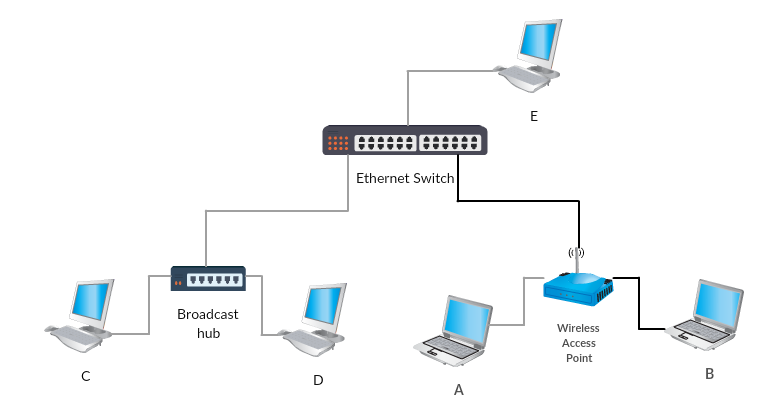
\includegraphics[scale = 0.5]{net} \\
\end{center}
\begin{itemize}
\item Hosts A and B are connected wirelessly to a wireless access point
\item Hosts C and D are connected to an old broadcast hub using wired Ethernet
\item The broadcast hub, wireless access point, and host E are connected to an Ethernet switch.
\end{itemize}

Assume that there is an active unencrypted TCP session between Hosts A and C and that every hosts on the network knows the IP address of A and C, which other host(s) on the network can passively eavesdrop on this communication?

\begin{solutionorbox}[1in]
+1 B, +1 D, -1 if mention E
\end{solutionorbox}

\part[2]
Based on the same topology from part (b), can any hosts passively eavesdrop on an unencrypted TCP session between A and B? If so, list the hosts that can eavesdrop on the communication, if not, briefly explain why not.

\begin{solutionorbox}[1in]
+1 NO +1 explanation: there is a switch between the wireless access point and all other hosts, so no one can passively eavesdrop on the session.
\end{solutionorbox}

\part[4]
Consider the following packet trace:\\

\begin{tabular}{|l|l|l|l|l|l|l|}
\hline
\textbf{timestamp} & \textbf{src\_ip} & \textbf{src\_port} & \textbf{dst\_ip} & \textbf{dst\_port} & \textbf{protocol} & \textbf{tcp\_flags}      \\ \hline
0.000000           & 164.124.33.78    & 34454              & 192.168.1.2      & 80                 & TCP               & {[}SYN{]}          \\ \hline
0.000001           & 192.168.1.2      & 80                 & 164.124.33.78    & 34454              & TCP               & {[}SYN{]}{[}ACK{]} \\ \hline
0.000002           & 38.198.26.9      & 24356              & 192.168.1.2      & 80                 & TCP               & {[}SYN{]}          \\ \hline
0.000003           & 192.168.1.2      & 80                 & 38.198.26.9    & 24356              & TCP               & {[}SYN{]}{[}ACK{]} \\ \hline
0.000004           & 76.196.6.157     & 6765               & 192.168.1.2      & 80                 & TCP               & {[}SYN{]}          \\ \hline
0.000005           & 192.168.1.2      & 80                 & 76.196.6.157    & 6765              & TCP               & {[}SYN{]}{[}ACK{]} \\ \hline
0.000060           & 189.109.37.180   & 34432              & 192.168.1.2      & 80                 & TCP               & {[}SYN{]}          \\ \hline
0.000061           & 192.168.1.2      & 80                 & 189.109.37.180    & 34432              & TCP               & {[}SYN{]}{[}ACK{]} \\ \hline
0.000064           & 189.109.30.67    & 43654              & 192.168.1.2      & 80                 & TCP               & {[}SYN{]}          \\ \hline
0.000065           & 192.168.1.2      & 80                 & 189.109.30.67    & 43654              & TCP               & {[}SYN{]}{[}ACK{]} \\ \hline
0.000136           & 132.212.36.112   & 8856               & 192.168.1.2      & 80                 & TCP               & {[}SYN{]}          \\ \hline
\end{tabular} \\

Based on this packet trace, answer the following questions:
\begin{enumerate}
\item What is the type of network attack shown in this trace?  
\item Specifically, what is the name of the attack? Briefly explain how you arrive at this conclusion.
\item What is the IP address of the victim?
\end{enumerate}

\begin{solutionorbox}[2in]
1. +1 denial of service \\
2. +1 TCP SYN flood; +1 Reason: Incomplete TCP handshake\\
3. +1 victim is 192.168.1.2
\end{solutionorbox}

\pagebreak

\part[4]
Consider the following packet trace:\\

\begin{tabular}{|l|l|l|l|l|l|l|}
\hline
\textbf{timestamp} & \textbf{src\_ip} & \textbf{src\_port} & \textbf{dst\_ip} & \textbf{dst\_port} & \textbf{protocol} & \textbf{tcp\_flags} \\ \hline
0.000000           & 189.109.37.180   & 34454              & 189.109.30.67    & 80                 & TCP               & {[}SYN{]}           \\ \hline
0.000001           & 189.109.30.67    & 80                 & 189.109.37.180   & 34454              & TCP               & {[}SYN{]}{[}ACK{]}  \\ \hline
0.000005           & 189.109.37.180   & 4538               & 189.109.30.67    & 22                 & TCP               & {[}SYN{]}           \\ \hline
0.000009           & 189.109.37.180   & 4652               & 189.109.30.67    & 443                & TCP               & {[}SYN{]}           \\ \hline
0.000010           & 189.109.30.67    & 443                & 189.109.37.180   & 4652               & TCP               & {[}SYN{]}{[}ACK{]}  \\ \hline
0.000016           & 189.109.37.180   & 8865               & 189.109.30.67    & 53                 & UDP               & n/a                 \\ \hline
0.000022           & 189.109.37.180   & 9575               & 189.109.30.67    & 21                 & TCP               & {[}SYN{]}           \\ \hline
\end{tabular} \\

Assume that TCP RST packets are omitted from the trace.  Based on this packet trace, answer the following questions:
\begin{enumerate}
\item What is the name of the network attack shown in this trace? Briefly explain how you arrive at this conclusion.
\item What are the application-layer protocol names of the services running on the victim's machine?
\item Name a tool that can be used to carry out this attack.
\end{enumerate}

\begin{solutionorbox}[2in]
1. +1 Port scanning, +1 many packets sent to common ports on the victim's IP without answers \\
2. +0.5 HTTP, +0.5 HTTPS or SSL or TLS\\
3. +1 nmap.  possibly other tools but not wireshark, aircrack, airmon, airodump, aireplay.
\end{solutionorbox}

\part[2]
In MP3.2, there was a task where you have to decrypt the SSL communication between the server and the client on the network by stealing the SSL private key from the server.  Now, assume that you do not have access to the private key file, what kind of attack could you launch against the client? Provide an example of the attack. 

\begin{solutionorbox}[1in]
The attacker can use ARP spoofing to trick the client into sending the credential to them instead of the server.  Other legitimate answers may be accepted.  All or nothing.
\end{solutionorbox}

\part[2]
Further, assume that all credential packets that you captured from part e) are for registration purposes, which means that the captured credentials are invalid unless they are received by the server.  If the server is only expecting the credentials from the client's ip address, what extra steps must you make in order to forward the captured credentials from your machine to the server? 

\begin{solutionorbox}[1in]
+2 Use IP spoofing to make the source IP of the packet be the client's before sending it to the server.  +1 partial if the answer mention changing the source IP without explicitly saying IP spoof.
\end{solutionorbox}


\end{parts}

\pagebreak

\titledquestion{Question \thequestion: AppSec MP Question (MP-specific)}  % -Gene

\begin{parts}

\part[4]

Consider the following function:

\begin{lstlisting}
void foo(char *arg)
{
   ... 
   char buf[32];
   strcpy(buf, arg);
}
\end{lstlisting}

\textbf{arg} is a pointer to a char string that is the command line input from the user.  
Make these assumptions:
\begin{itemize}
\item The machine is a 32-bit little-endian system that behaves like the VM from MP4.
\item All the defences mentioned in lectures are off
\item You see the following information when the program arrives to the breakpoint at foo that you set earlier with the command \texttt{break foo} :
\begin{itemize}
\item \textbf{buf} begins at 0xbffebfa0. 
\item $(gdb)$  x/2wx \$ebp\\
0xbffebfd8: 0xbffec064 0x08048fe5
\end{itemize}
\end{itemize}



Describe parts of the input (\textbf{arg}) that you would give to the program to overflow the buffer (\textbf{buf}) and execute the same shellcode that was given for the MP. The file shellcode.py has size of 23 bytes. Be specific and include exact numbers.

\begin{solutionorbox}[2in]
shellcode + 0xd8-0xa0+4-23 = 37 bytes of 'A' or junk + 0xbffebfa0 (start of buffer, where shellcode is)

+1 including shellcode
+2 return addr at the correct location (60 bytes then return addr)
+1 return addr has correct value (to shellcode)

\end{solutionorbox}

\part[2]

Continue from part(a): if instead, you see the following information when the program arrives to the breakpoint at foo that you set earlier with the command \texttt{break foo} :
\begin{itemize}
\item \textbf{buf} begins at 0xbffebfa0. 
\item $(gdb)$  x/2wx \$ebp\\
0xbffebfd8: 0xbffec064 0x08034586
\end{itemize}

Would you need to change your solution from part(a) to achive the same goal? Explain your answer.

\begin{solutionorbox}[1in]

+1 NO
+1 Changing the legit return addr is irrelavant to where your shellcode is

\end{solutionorbox}


\pagebreak
\part[4]

Consider the following gadgets. The first column is the address in hexadecimal representation, and the second column is the instruction at that address:

\begin{verbatim}
8051750:	xor    %eax,%eax 
8051752:	ret  

8058680:	cmp    $0xffffff83,%eax
8058683:	jne    80586f8 <_exit>
8058689:	mov    %eax,(%ecx)
805868f:	ret   

8058679:	mov    %ecx,(%eax)
805867f:	ret   

8057360:        pop    %edx
8057361:	pop    %ecx
8057362:	pop    %ebx
8057363:	ret  

8057ae0:	int    $0x80
\end{verbatim}

Assume these are the only gadgets that you can use, how would you set the value at memory address 0xbffe3222 to be 0x00000000 (a null pointer)? Draw a picture of the stack showing how you would chain the gadgets. (Label the location of the original return address and label which way is the top/bottom of the stack)

\begin{solutionorbox}[3in]
top of stack \\
0x8051750 \#set eax to 0 (original return address) \\
0x8057361 \#pop ecx and ebx \\
0xbffe3222 \#ecx value \\
0xanything \#ebx value \\
0x8058689 \#mov 0 in eax to mem[ecx] which is 0xbffe3222

-2 if answer contains 8058680, 8058683, 8057ae0, or 8058679 (undefined behavior)
-2 if answer doesn't have enough values on the stack to pop to registers
+1 sets eax to 0
+1 pops 0xbffe3222 to ecx
+2 mov eax to mem[ecx]

\end{solutionorbox}

\part[4]
Continue from part(c): assume the value at memory address 0xbffe3222 is originally 0xc0a8ea66, and you want to change the value to 0x00000066. How do you need to modify your answer from part(c) to achieve this goal?

\begin{solutionorbox}[1in]
+4 modify the value for pop ecx instruction to be 0xbffe3223 or +2 mentioning little endian or +1 using a modified value for ecx but wrong address
\end{solutionorbox}

\pagebreak

\part[2]

Why would one want to use a callback shell(4.2.10) as the payload instead of a regular shell(shellcode.py)?

\begin{solutionorbox}[1in]
The attacker will be able to control the machine over a network instead of just locally. 2 points all or nothing

\end{solutionorbox}

\part[2]

If ASLR was on for MP4.2, would your answers still work? Why?

\begin{solutionorbox}[1in]
+1 NO
+1 Return addr and payload addr are randomized 

\end{solutionorbox}

\end{parts}

\pagebreak

\titledquestion{Question \thequestion: Forensics MP Question} % -Leslie

From the incident introduced in MP5, you have investigated victim's
and one of the suspects' machine through two different checkpoints.
To get a comprehensive understanding, police department collected one
more possibly relevant disk image. Do you remember the chat history of
the victim's machine? Investigators obtained the hard disk of
``alice.innocuous's'' machine.

This disk image was uploaded to the digital forensics department's
server. Bob was recently hired in the digital forensics team and was
given this as his first case to investigate. As he started to
investigate, he was so excited and booted the hard disk on a machine,
selected a disk partition, and started to explore. He navigated
through the system's directories, opened a few log files to look for
the relevant evidence, and ran some command lines. Then, he realized
something was wrong.

Fortunately, a more experienced expert, Cathy, duplicated the original
disk images before Bob started investigating. Through Autopsy, she
extracted few files that might be relevant to the case. \textbf{Part
  of the files are provided on the next page(s)} which are based on
the same time zone setting as the setting of the user's machine.

\begin{parts}

\part[1]
For a downloaded disk image, how can you verify the disk image is the original and not corrupted during the download?

\begin{solutionorbox}[1in]
Compare the checksum, hash values (MD5, SHA-1) of the disk images usually provided with the download file.
\end{solutionorbox}

\part[2]
What are the two main results that Bob's action can lead to? 

\begin{solutionorbox}[1in]
[1 point] tampering of the data: e.g. last accessed time of the file gets changed, bash history gets overwritten
    [1 point] suspect may have pre-setup the partition to prevent from live analysis (obfuscate with other OS partition, disk wiping etc.)
(optional) attacking of the system is maybe needed to log on
\end{solutionorbox}

\part[1]
What is the computer name?

\begin{solutionorbox}[1in]
alice-personal. /etc/hostname contains the computer name.
\end{solutionorbox}

\part[1]
Where in the file system can you find installed OS information? List one of the options through dead analysis.

\begin{solutionorbox}[1in]
/etc/issue or /etc/lsb-release
\end{solutionorbox}

\pagebreak

\part[1]
What is the timezone setting of the system?

\begin{solutionorbox}[1in]
EST. Time setting in New York city.
\end{solutionorbox}

\part[1]
Who was the last logon user on the system?

\begin{solutionorbox}[1in]
alice.innocuous. obtained from /var/log/auth.log
\end{solutionorbox}

\part[2]
What is the IP address of the attacker? What is the IP address of the user's machone during the attack?

\begin{solutionorbox}[1in]
[1 point] 10.46.1.105 and [1 point] unknown
\end{solutionorbox}

\part[2]
List all the usernames of the account the attacker tried and used to connect through SSH.

\begin{solutionorbox}[1in]
[1 point] l33th4x0r and [1 point] root
\end{solutionorbox}

\part[2]
There is a trace of remote access attack in this machine. During the attack, the attacker used brute-force method with 6-digits password (digits: $0 \sim 9$ numeric values) and successfully cracked. Assuming that 10 passwords can be tried in 1 millisecond, 1) how long will it take in the worst case scenario? Express in X minutes Y seconds. 2) What was the actual number of passwords tried before successfully cracking, i.e. number of failed attempts?

\begin{solutionorbox}[1in]
[1 point] $10^6$ combinations of password possible. (1000000 passwords)/(10 passwords/1 millisecond) = 100000 milliseconds = 100 seconds = 1 min 40 seconds.
[1 point] From the log file /var/log/auth.log, failed login attempts from suspect was 6.
\end{solutionorbox}

\pagebreak

\part[1]
What application was used for e-mail communication by the attacker?

\begin{solutionorbox}[1in]
Mozilla Thunderbird
\end{solutionorbox}

\part[1]
What was the e-mail account used by the attacker?

\begin{solutionorbox}[1in]
alice.innocuous.1996@gmail.com
\end{solutionorbox}

\part[2]
Who made the searches in browsing email inbox? What was the keyword used in the search?

\begin{solutionorbox}[1in]
[1 point] alice.innocuous (the original user) and [1 point] keyword is ladiesman.
\end{solutionorbox}

\part[3]
What were the attacker's main activities of the obtained hard disk? Explain concisely in time order. List at most 5 activities.

\begin{solutionorbox}[3in]
Account was remotely logged on. Searched and read chat history with victim. Added alice.innocuous email account into root. Email logged in using Thunderbird. Email was composed to ladiesman461@gmail.com. Connection closed.
\end{solutionorbox}

\end{parts}

\pagebreak

\begin{lstlisting}
|\textbf{<Hard Disk>}|
|\textbf{File path: /etc/hostname}|
alice-personal

|\textbf{File path: /etc/hosts}|
127.0.0.1   localhost
127.0.1.1   alice-personal

# The following lines are desirable for IPv6 capable hosts
::1        ip6-localhost ip6-loopback
fe00::0    ip6-localnet
ff00::0    ip6-mcastprefix
ff02::1    ip6-allnodes
ff02::2    ip6-allrouters

|\textbf{File path: /etc/issue}|
Ubuntu 14.04.3 LTS \n \l

|\textbf{File path: /etc/lsb-release}|
DISTRIB_ID=Ubuntu
DISTRIB_RELEASE=14.04
DISTRIB_CODENAME=trusty
DISTRIB_DESCRIPTION="Ubuntu 14.04.3 LTS"

|\textbf{File path: /etc/timezone}|
America/New_York

|\textbf{File path: /etc/localtime}|
...
EST5EDT,M3.2.0,M11.1.0

|\textbf{File path: /home/alice.innocuous/.bash\_history}|
<Access Time>   2015-11-07 10:32:44
<Modify Time>   2015-11-07 10:32:44
<Change Time>   2015-11-07 10:32:44
...
firefox &
shutdown -h now
...

|\textbf{File path: /home/alice.innocuous/.ssh/known\_hosts}|
99.118.111.49
141.212.111.41

|\textbf{File path: /home/alice.innocuous/.thunderbird/ImapMail/imap.gmail.com/[Gmail]/Sent Mail}|
<E-Mail To>       ladiesman461@gmail.com
<E-Mail From>     alice.innocuous.1996@gmail.com
<Date Sent>       2015-11-03 16:01:46 EST
<Message>         Hey, I think we should...
<Subject>         Hey-           

\end{lstlisting}

\pagebreak

\begin{lstlisting}

|\textbf{File path: /root/.bash\_history}|
<Access Time>   2015-11-03 16:07:31
<Modify Time>   2015-11-03 16:07:31
<Change Time>   2015-11-03 16:07:31
pwd
cd /home
ls
cd alice.innocuous
ls -a
cd ./purple/log/jabber/alice.innocuous@jwchat.org
ls
cd ladiesman461@jwchat.org
open 2015-11-02.204322-0500EST.html
open 2015-11-03.104811-0500EST.html
firefox
sudo mail
sudo adduser alice.innocuous mail
thunderbird
thunderbird -compose "to=ladiesman461@gmail.com"
exit

\end{lstlisting}

\pagebreak

\begin{lstlisting}

|\textbf{File path: /var/log/auth.log}|
...
Oct 30 17:02:30 alice-personal login: session opened for user alice.innocuous by LOGIN(uid=0)
Oct 30 17:02:32 alice-personal login: ALICE.INNOCUOUS LOGIN ON 'tty1'
...
Oct 30 18:01:20 alice-personal sshd: server listening on :: port 22
...
Oct 30 18:53:05 alice-personal sshd: server listening on :: port 22
Oct 30 19:02:10 alice-personal lightdm: session closed for user alice.innocuous by lightdm(uid=0)
...
Nov 3 15:20:20 alice-personal sshd: Invalid user l33th4x0r from 10.46.1.105
Nov 3 15:23:20 alice-personal sshd: authentication failure; rhost=10.46.1.105, ruser=root
Nov 3 15:40:20 alice-personal sshd: Failed password for root from 10.46.1.105 port XXXX ssh2
Nov 3 15:40:20 alice-personal sshd: Failed password for root from 10.46.1.105 port XXXX ssh2
Nov 3 15:40:21 alice-personal sshd: server listening on :: port 22
Nov 3 15:40:21 alice-personal sshd: Failed password for root from 10.46.1.105 port XXXX ssh2
Nov 3 15:40:21 alice-personal sshd: Failed password for root from 10.46.1.105 port XXXX ssh2
Nov 3 15:40:21 alice-personal sshd: Failed password for root from 10.46.1.105 port XXXX ssh2
Nov 3 15:40:22 alice-personal sshd: Failed password for root from 10.46.1.105 port XXXX ssh2
Nov 3 15:40:28 alice-personal sshd: server listening on :: port 22
Nov 3 15:40:29 alice-personal sshd: Accepted password for root from 10.46.1.105 server listening on :: port 22
Nov 3 15:41:00 alice-personal sshd: pam_unix(sshd:session): session opened for user root by (uid=0)
Nov 3 15:41:01 alice-personal systemd: pam_unix(systemd:session): session opened for user root by (uid=0)
...
Nov 3 16:07:31 alice-personal sshd: pam_unix(sshd:session): session closed for user root by (uid=0)
...
Nov 4 18:53:05 alice-personal sshd: server listening on :: port 22
Nov 5 17:02:30 alice-personal login: session opened for user alice.innocuous by LOGIN(uid=0)
Nov 5 17:02:32 alice-personal login: ALICE.INNOCUOUS LOGIN ON 'tty1'

\end{lstlisting}

\pagebreak

\begin{lstlisting}

|\textbf{File path: /home/alice.innocuous/.mozilla/firefox/places.sqlite}|
<Date Accessed>   <Strings (Contents)>   
Oct 30 17:15:00 https://mail.google.com/
Oct 30 17:15:24 https://mail.google.com/mail/u/0/#inboxInbox (54) - alice.innocuous.1996@gmail.com - Gmail...
Oct 30 17:17:48 https://mail.google.com/mail/u/0/#inbox/14d2816b7a04c3ff
Oct 30 17:20:02 https://www.google.com/search?q=party+costumes&oq=party+costumes&aqs=firefox..69i57j0l5.7255j0j7&sourceid=firefox&ex_sm=119&ie=UTF-8
Oct 30 18:15:00 https://mail.google.com/mail/u/0/#inboxInbox (53) - alice.innocuous.1996@gmail.com - Gmail...
Oct 30 18:15:18 https://mail.google.com/mail/u/0/#search/ladiesman
Oct 30 18:15:39 https://mail.google.com/mail/u/0/#search/from%3A+ladiesman461%40gmail.com/14d2816b7a04c3ffHey! Let's hang out together some day - ladiesman461@gmail.com - Gmail...
Oct 30 18:25:31 https://mail.google.com/mail/u/0/#inbox?compose=new
Oct 30 18:25:49 https://mail.google.com/mail/u/0/#inbox?compose=new=24987sdf98q3123
Oct 30 18:35:50 https://mail.google.com/mail/u/0/#inbox/14d2816b7a04c3ff
Oct 30 18:55:17 https://mail.google.com/mail/u/0/#trashTrash - alice.innocuous.1996@gmail.com - Gmail
Oct 30 19:01:00 https://mail.google.com/mail/LogOut?...
Nov 3 15:50:00  https://mail.google.com/

\end{lstlisting}

\end{questions}

\end{document}
